\documentclass{elsarticle}

% Use the option doublespacing or reviewcopy to obtain double line spacing
% \documentclass[doublespacing]{elsart}

% the natbib package allows both number and author-year (Harvard)
% style referencing;
\usepackage{natbib}

% if you use PostScript figures in your article
% use the graphics package for simple commands
% \usepackage{graphics}
% or use the graphicx package for more complicated commands
% \usepackage{graphicx}
% or use the epsfig package if you prefer to use the old commands
% \usepackage{epsfig}

% The amssymb package provides various useful mathematical symbols
\usepackage{amssymb}
\usepackage{amsmath}
\usepackage{amsthm}
\usepackage{mathtools}

% The lineno packages adds line numbers. Start line numbering with
% \begin{linenumbers}, end it with \end{linenumbers}. Or switch it on
% for the whole article with \linenumbers.
% \usepackage{lineno}

% \linenumbers

\newcommand{\X}{\mathbf{X}  }
\newcommand{\Xe}{\mathbf{X}_e  }
\newcommand{\XeT}{\mathbf{X}_e^{\top}}

\newcommand{\ye}{\begin{bmatrix} \mathbf{y}  \\ \mathbf{y}_u \end{bmatrix}}
\newcommand{\G}{\left(\Xe^T \Xe \right)^{-1}}
\newcommand{\missidentity}{\begin{bmatrix} 0 & 0 \\ 0 & \textbf{I }\end{bmatrix}}
\newcommand{\Greg}{\left(\Xe^{\top} \Xe + \lambda \missidentity \right)^{-1}}
\newcommand{\Cb}{\mathcal{C}_{\beta}}

\newtheorem{theorem}{Theorem}
\newproof{pf}{Proof}

\begin{document}

\begin{frontmatter}

% Title, authors and addresses

% use the thanksref command within \title, \author or \address for footnotes;
% use the corauthref command within \author for corresponding author footnotes;
% use the ead command for the email address,
% and the form \ead[url] for the home page:
% \title{Title\thanksref{label1}}
% \thanks[label1]{}
% \author{Name\corauthref{cor1}\thanksref{label2}}
% \ead{email address}
% \ead[url]{home page}
% \thanks[label2]{}
% \corauth[cor1]{}
% \address{Address\thanksref{label3}}
% \thanks[label3]{}

\title{Implicitly Constrained Semi-Supervised Least Squares Classification}

\author[lumc,prlab]{Jesse H. Krijthe}
\author[prlab,copenhagen]{Marco Loog}

\address[lumc]{Department of Molecular Epidemiology, Leiden University Medical Center}
\address[prlab]{Pattern Recognition Laboratory, Delft University of Technology}
\address[copenhagen]{The Image Group, University of Copenhagen}

\begin{abstract}
We introduce a novel semi-supervised version of the least squares classifier. 
This implicitly constrained least squares (ICLS) classifier minimizes the squared loss on the labeled data among the set of parameters implied by all possible labelings of the unlabeled data.
Unlike previous discriminative semi-supervised methods, our approach does not introduce explicit additional assumptions into the objective function, but leverages implicit assumptions already present in the choice of the supervised least squares classifier.  
We show this classifier can be formulated as a quadratic programming problem and its solution can be found using a simple gradient descent procedure. 
In the case of a 1-dimensional feature vector without intercept, we give an intuitive proof that this method can never lead to worse performance than supervised least squares classification in terms of the squared loss criterion used in least squares classification. 
Experimental results corroborate the theoretical results and indicate desirable properties over alternative semi-supervised approaches to least squares classification. 
\end{abstract}

\begin{keyword}
% keywords here, in the form: keyword \sep keyword
Semi-supervised learning \sep Least Squares Classification \sep Constrained Learning
% PACS codes here, in the form: \PACS code \sep code
\end{keyword}

\end{frontmatter}

% main text
\section{Introduction}
\label{section:Introduction}
Semi-supervised classification concerns the problem of using additional unlabeled data, aside from only labeled data considered in supervised learning, to learn a classification function that maps objects to a correct target class as closely as possible.
In the supervised paradigm this mapping is learned using a set of $N_l$ examples $(\mathf{x}_i,y_i)$, where $\mathf{x}_i$ is a feature vector and $y_i$ a corresponding label.  In the semi-supervised scenario we are given an additional and often large set of $N_u$ unlabeled objects $(\mathf{x}_i)$. 
The challenge of semi-supervised learning is to incorporate this additional information to improve the classification function over the function one would find using only the labeled data.

The goal of this work is to build a semi-supervised version of the least squares classifier that has the property that, at least in expectation, its performance is not worse than supervised least squares classification.
While it may seem like an obvious requirement for any semi-supervised method, current approaches to semi-supervised learning do not have this property. 
In fact, performance can significantly degrade as more unlabeled data is added, as has been shown in \cite{Cozman2006}. 
Additionally, many semi-supervised learning procedures are formulated as non-convex objective functions which are hard to optimize. 
A more satisfactory state of affairs would therefore be computationally efficient methods that on average do not lead to worse classification performance than their supervised alternatives.

In this work, we present a novel approach to semi-supervised learning for the least squares classifier. 
We will refer to this approach as implicitly constrained semi-supervised learning (ICLS). 
The goal is to leverage the implicit assumptions present in supervised least squares classification to construct a semi-supervised version. 
That is, we exploit constraints inherent in the choice of the supervised classifier, whereas current state-of-the-art semi-supervised learning approaches typically rely on imposing additional extraneous, and possibly incorrect, assumptions \cite{Seeger2001,Singh2008}.

In least squares classification, classes are encoded as numerical outputs after which a linear regression model is applied (see Section \ref{section:leastsquares}). By placing a threshold on the output of this model, we can use the linear function to predict class labels. 
In a different neural network formulation, this classifier is also known as Adaline \cite{Widrow1960}.
There are several reasons why this is a particularly interesting classifier to study: 
First of all, the least squares classifier is a discriminative classifier. 
Some have claimed semi-supervised learning without additional assumptions is impossible for discriminative classifiers \cite{Seeger2001,Singh2008}. 
Our results, like \cite{Sokolovska2008}, show this may not strictly hold. 
Secondly, as we will show in section \ref{section:icls}, the closed-form solution for the supervised least squares classifier allows us to study its theoretical properties.
Moreover, using the closed-form solution we can rewrite our semi-supervised approach as a quadratic programming problem, which can be solved through a simple gradient descent with boundary constraints. 
Lastly, least squares classification is a useful and adaptable classification technique  allowing for straightforward use of, for instance, regularization, sparsity penalties or kernelization \cite{Hastie2001,Rifkin2003,Tibshirani1996,Poggio2003}. 
Using these formulations, it has been shown to be competitive with state-of-the-art methods based on loss functions other than the squared loss \cite{Rifkin2003} as well as computationally efficient on large datasets \cite{Bottou2010}.

The proposed semi-supervised least squares classifier works by constraining the solution of the supervised least squares classifier based on the unlabeled data. 
These constraints follow from the choice of the supervised classifier and require only minimal additional assumptions.
In the univariate setting without intercept and assuming perfect knowledge of $p(\mathbf{x})$ we show this procedure \emph{never} gives worse performance in terms of the squared loss criterion compared to the supervised least squares classifier. 
In our experiments, we indeed find that this new approach displays many properties we deem desirable in a semi-supervised learner, namely that it quickly converges to a global optimum and that on average performance increases as we increase the amount of unlabeled data.

The main contributions of this paper are

\begin{itemize}
  \item A novel convex formulation for robust semi-supervised learning under squared loss (Equation \eqref{icls})
  \item An intuition through a proof of non-degradation for the 1-dimensional case (Theorem \ref{theorem:1d})
  \item An empirical evaluation of the properties of this classifier (Section \ref{section:empiricalresults})
\end{itemize}

The rest of this paper is organized as follows. 
Section \ref{section:relatedwork} discusses related work on semi-supervised learning. 
Section \ref{section:method} introduces our semi-supervised version of the least squares classifier. 
We then derive a quadratic programming formulation and present a simple way to solve this problem through bounded gradient descent. 
Section \ref{section:theoreticalresults} contain a proof of the improvement of the ICLS classifier over the supervised alternative. 
Section \ref{section:empiricalresults} presents an empirical evaluation of the proposed approach on benchmark datasets. The final sections discuss the results and conclude.

\section{Related Work} 
\label{section:relatedwork}
Many diverse semi-supervised learning techniques have been proposed \cite{Chapelle2006,Zhu2009}. 
While these have proven successful in  particular applications, such as document classification \cite{Nigam2000}, it has also been observed that these techniques may give worse performance than their supervised counterparts \cite{Cozman2003,Cozman2006}. 
In these cases, disregarding the unlabeled data would lead to better performance. 
Some \cite{Goldberg2009,Wang2007a} have argued that \emph{agnostic} semi-supervised learning, which \cite{Goldberg2009} define as semi-supervised learning that is at least no worse than supervised learning, can be achieved by cross-validation on the limited labeled data. 
Agnostic semi-supervised learning follows if we only use semi-supervised methods when their estimated cross-validation error is significantly lower than those of the supervised alternatives.
As the results of  \cite{Goldberg2009} indicate, this criterion may be too conservative: given the small amount of labeled data, a semi-supervised method will only be preferred if the difference in performance is very large. 
If the difference is less distinct, the supervised learner will always be preferred and we potentially ignore useful information from the unlabeled objects. 
Moreover, this cross-validation approach can be computationally demanding. 
The method considered in our work is different from most previous work in smei-supervised learning in that it is inherently robust against this degradation in performance.

A simple approach to semi-supervised learning is offered by the self-learning procedure \cite{McLachlan1975}, also known as Yarowsky's algorithm \cite{Yarowsky1995,Abney2004}. 
Taking any classifier, we first estimate its parameters on only  the labeled data. 
Using this trained classifier we label the unlabeled points and add them, or potentially only those we are most confident about, with their predicted labels to the labeled training set. 
The classifier parameters are re-estimated using these labeled objects to get a new classifier. 
One iteratively applies this procedure until the predicted labels of the unlabeled data no longer change.

One of the advantages of this procedure is that it can be applied to any supervised classifier.
It has also shown practical success in some application domains, particularly document classification \cite{Nigam2000,Yarowsky1995}. 
Unfortunately, the process of self-training can also lead to severely decreased performance, compared to the supervised solution \cite{Cozman2003,Cozman2006}. 
One can imagine that once an object is incorrectly labeled and added to the training set, its incorrect label may be reinforced, leading the solution away from the optimum. 
Self-learning is closely related to the expectation maximization (EM) based approaches \cite{Abney2004}. Indeed, expectation maximization suffers from the same issues as self-learning \cite{Zhu2009}.
In Section \ref{section:empiricalevaluation} we have included self-learing with the least squares classifier in the performance comparison.

More recent work in semi-supervised learning has focused on introducing useful assumptions about the unlabeled data that can help link information about the distribution of the features $P(\mathbf{x})$ to the posterior of the classes $P(y|\mathbf{x})$.
Commonly used assumptions are the smoothness assumption, objects that are close in the feature space likely share the same label; the cluster assumption, objects in the same cluster share a label; and the low density assumption enforcing that the decision boundary should be in a region of low density. 

%  In the case of logistic regression, entropy regularization can be applied by adding an additional term to the objective function that encodes the entropy of the classifier in the unlabeled points. Unfortunately, the new objective is hard to minimize. Some work has been done to do this more efficiently for particular models \cite{Mann2007}.

The low-density assumption is used in entropy regularization \cite{Grandvalet2005} as well as for support vector classification in the transductive support vector machine (TSVM)  \cite{Joachims1999}. 
When used in the semi-supervised setting this is closely related to the formulation of S$^3$VM \cite{Bennett1998,Sindhwani2006}. 
Like in entropy regularization, for the semi-supervised versions of SVM, an additional term is added to the objective function to push the decision boundary away from dense regions. 
The resulting objective function is non-convex, owing to the possible labelings that can be assigned to the unlabeled objects. 
Several approaches have been put forth to solve this difficult optimization problem, such as the convex concave procedure \cite{Collobert2006} and difference convex programming \cite{Sindhwani2006,Wang2007}.

Some have argued unlabeled data can \emph{only} help if $P(\mathbf{x})$ and $P(y|\mathbf{x})$ are somehow linked \cite{Singh2008}.
One of the results in our work is that in some cases (i.e. the least squares classifier) we do not need explicit assumptions about those links for semi-supervised learning to be possible. 
Instead, we leverage the implicit assumptions, including possible model misspecification, that are already present in the supervised classifier.

In the approaches presented above, a parameter controls the importance of the unlabeled points. When the parameter is correctly set, it is clear, as \cite{Wang2007a} claims, that TSVM is always no worse than supervised SVM. 
It is, however, non-trivial to choose this parameter, given that semi-supervised learning is most interesting in cases where we have limited labeled objects, making a choice using cross-validation very unstable. 
In practice, therefore, TSVM can also lead to worse performance than the supervised support vector machine. 
\cite{Li2011} tries to guard against this deterioration by proposing safe semi-supervised SVM (S4VM). 
In some way, this method tries to find the safest decision boundary among all low-density decision boundaries identified by S3VM. 
While the approach is often successful in protecting against deterioration when compared to supervised SVM, the price to pay is smaller performance increases on many datasets as well as significantly higher computational cost.

\cite{Loog2014b,Loog2014a} attempt to guard against the possibility of deterioration in performance by not introducing additional assumptions, but instead leveraging implicit assumptions already present in the choice of the supervised classifier. 
These assumptions link parameters estimates that depend on labeled data to parameter estimates that rely on all data. 
By exploiting these links, semi-supervised versions of the nearest mean classifier and the linear discriminant are derived. 
Because these links are unique to each classifier, the approach does not generalize directly to other classifiers. 
The method presented here is similar in spirit, but unlike \cite{Loog2014b,Loog2014a}, no explicit equations have to be formulated to link parameter estimates using only labeled data to parameter estimates based on all data. 
This makes the current approach more flexible.

Little work has been done on applying semi-supervised learning to the least squares classifier specifically. 
For least squares regression, \cite{Shaffer1991} studied the value of knowing $\mathbb{E}[\mathbf{X}'\mathbf{X}]$, where $\mathbf{X}$ is the $N_l \times m$ design matrix containing the feature values for each observation. 
If we assume the number of unlabeled data points is large, this is similar to the semi-supervised situation. 
It is shown that if the size of the parameters is small compared to the noise, the variance of a estimator that plugs in $\mathbb{E}[\mathbf{X}'\mathbf{X}]$ as the estimate of $\mathbf{X}'\mathbf{X}$ in the closed form solution for ordinary least squares regression, is lower  than ordinary least squares regression.  
As the size of the parameters increases, this effect reverses. 
In fact, the paper demonstrates that in this semi-supervised setting no best linear unbiased estimator for the regression coefficients exists. 
In Section \ref{section:empiricalresults}, we compare our approach to using this plug-in estimate by substituting the matrix $\mathbf{X}'\mathbf{X}$ by a version based on both labeled and unlabeled data. 
A similar plug-in procedure has been used by \cite{Fan2008} for the dimensionality reduction technique that often is referred to as linear discriminant analysis. Here the (normalized) total scatter matrix, which plays a similar role to the $\mathbf{X}'\mathbf{X}$ matrix in least squares regression is exchanged with the more accurate estimate of the total scatter based on both labeled and unlabeled data.

\section{Implicitly Constrained Least Squares Classification}
\label{section:method}
Given a limited set of $N_l$ labeled objects and a potentially large set of $N_u$ unlabeled objects, the goal of implicitly constrained least squares classification is to use the latter to improve the solution of the least squares classifier trained on just the labeled data. We start with a sketch of this approach, before discussing the details.

\begin{figure}[ht] 
  \centering
      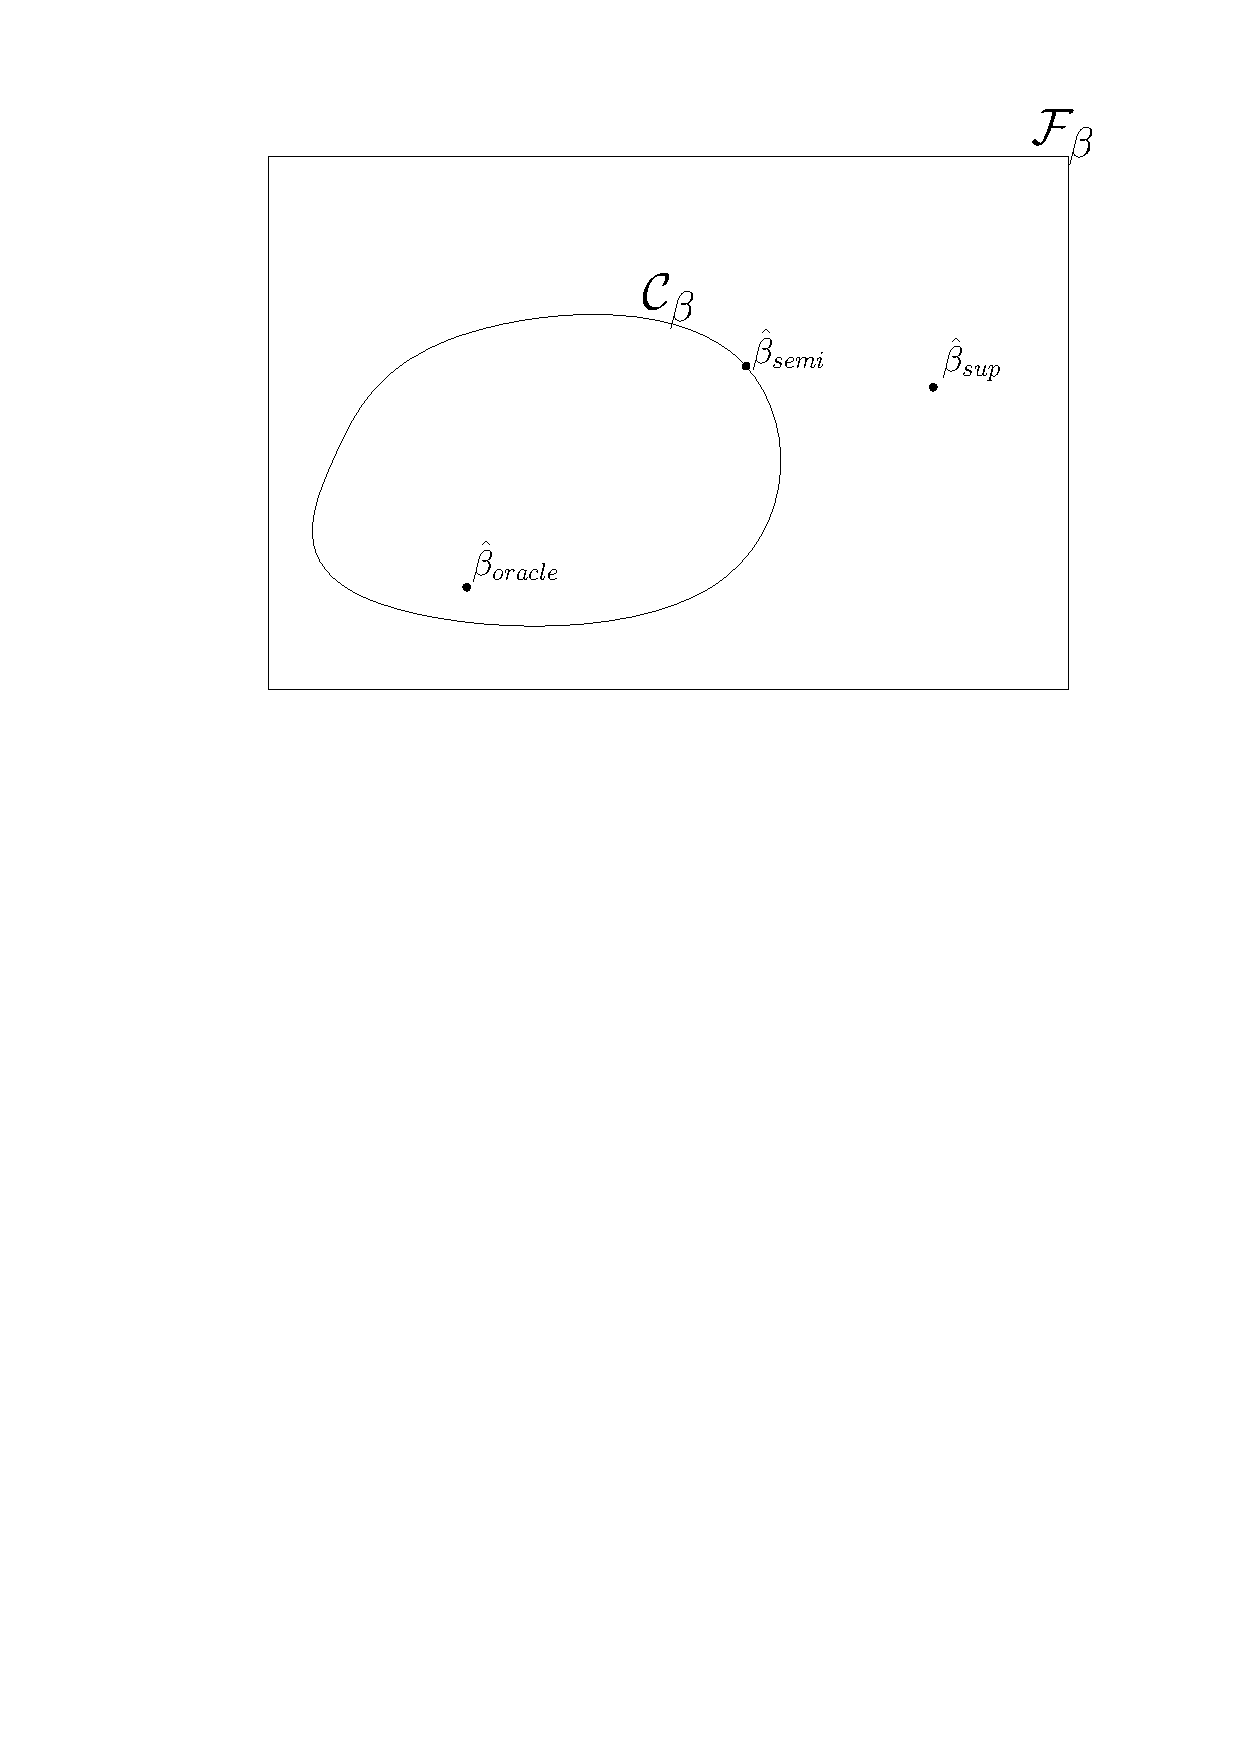
\includegraphics[width=0.5\textwidth]{constrainedspace.pdf}
  \caption{A visual representation of implicitly constrained semi-supervised learning. $\mathcal{F}_{\beta}$ is the space of all linear models. $\hat{\beta}_{sup}$ denotes the solution given only a small amount of labeled data. $\mathcal{C}_{\beta}$ is the subset of the space which contains all the solutions we get when applying all possible (soft) labelings to the unlabeled data. $\hat{\beta}_{semi}$ is a projection of $\hat{\beta}_{sup}$ onto $\mathcal{C}_{\beta}$. $\hat{\beta}_{oracle}$ is the supervised solution if we would have the labels for all the objects.} \label{fig:constrainedsubset}
\end{figure}

Given the supervised least squares classifier, consider the hypothesis space of all possible parameter vectors, which we will denote as $\mathcal{F}_{\beta}$, see Figure \ref{fig:constrainedsubset}. Given a set of labeled objects, we can determine the supervised parameter vector $\hat{\beta}_{sup}$. Suppose we also have a potentially large number $N_u$ of unlabeled objects. Assume that these object have a label, it is merely unknown to us. If these labels were to be revealed, it is clear how the additional objects can improve classification performance: we estimate the least squares classifier using all the data to obtain the parameter vector $\hat{\beta}_{oracle}$. Since this estimate is based on more objects, we expect the parameter estimate to be better. These real labels are unknown, but we can still consider all possible labelings of unlabeled objects, and estimate corresponding parameters based on these imputed labelings. In this way, we get a set of possible parameters for our classifier, which form the set denoted by $\mathcal{C}_{\beta} \subset \mathcal{F}_{\beta}$. Clearly one of these labelings corresponds to the real, but unknown, labeling, so one of the parameter estimates in this set corresponds to the solution we would obtain using all the correct labels of both the labeled and unlabeled objects. Because these are the only possible classifiers when the true labels would be revealed, we propose to look within this set $\mathcal{C}_{\beta}$ for an improved semi-supervised solution. 

Two issues then remain: how do we choose the best parameters from this set and how do we find these without having to enumerate all possible labelings?

Looking at the first problem, we reiterate that the goal of semi-supervised learning is to find a good classification rule and, therefore, still the obvious way to evaluate this rule is by the loss on the labeled training points. In other words, we choose the classifier from the parameter set that minimizes the loss on the labeled points. Note this approach is rather different from other approaches to semi-supervised learning where the loss is adapted by including a term that depends on the unlabeled data points. In our formulation, the loss function is still the regular, supervised loss of our classification procedure. We will denote this solution by $\hat{\beta}_{semi}$.

As for the second issue, after relaxing the constraint that we need hard labels for the data points, we can derive the gradient of the loss on the labeled training points with respect to the imputed labels of the unlabeled objects. This will allow us to find the optimal labeling through a simple gradient descent procedure without having to go through all possible labelings of the unlabeled data. 

\subsection{Multivariate Least Squares Classification} \label{section:leastsquares}

Least squares classification \cite{Hastie2001,Rifkin2003} is the direct application of well-known ordinary least squares regression to a classification problem. A linear model is assumed and the parameters are minimized under squared loss. Let $\mathbf{X}$ be an $N_l \times (m+1)$ design matrix with $N_l$ rows containing vectors of length equal to the number of features $m$ plus a constant feature to encode the intercept. Vector $\textbf{y}$ denotes an $N_l \times 1$ vector of  class labels. We encode one class as $0$ and the other as $1$.  The multivariate version of the empirical risk function for least squares regression is given by

\begin{equation} \label{squaredloss}
\hat{R}(\beta) = \frac{1}{n} \left\|  \mathbf{X} \boldsymbol{\beta}-\mathbf{y} \right\| _2^2
\end{equation}
The well known closed-form solution for this problem is found by setting derivative with respect to $\boldsymbol{\beta}$ equal to $\textbf{0}$ and solving for $\boldsymbol{\beta}$, giving:

\begin{equation} \label{olssolution}
\boldsymbol{\hat{\beta}}=\left(\mathbf{X}^T \mathbf{X}\right)^{-1} \mathbf{X}^T \mathbf{y}
\end{equation}

In case $\textbf{X}^T \textbf{X}$ is not invertible (for instance when $n<(m+1)$), a pseudo-inverse is applied. As we will see, the convexity and subsequent closed form solution to this problem will enable us to formulate our semi-supervised learning approach in terms of a standard quadratic programming problem.

\subsection{Implicitly Constrained Least Squares Classification} \label{section:icls}

In the semi-supervised setting, apart from a design matrix $\textbf{X}$ and target vector $\textbf{y}$, an additional set of measurements $\textbf{X}_u$ of size $N_u \times (m+1)$ \emph{without} a corresponding target vector $\textbf{y}_u$ is given. In what follows, $\mathbf{X}_e=\begin{bmatrix} \mathbf{X}^T  & \mathbf{X}_u^T \end{bmatrix}^T$ denotes the extended design matrix which is simply the concatenation of the design matrices of the labeled and unlabeled objects.

In the implicitly constrained approach, we propose that a sensible solution to incorporate this additional information is to search within the set of classifiers that can be obtained by all possible labelings $\textbf{y}_u$, for the one classifier that minimizes the \emph{supervised} empirical risk function \eqref{squaredloss}. This set, $\mathcal{C}_{\boldsymbol{\beta}}$, is formed by the $\boldsymbol{\beta}$'s that would follow from training supervised classifiers on all (labeled and unlabeled) objects going through all possible soft labelings for the unlabeled samples, i.e., using all $\textbf{y}_u \in [0,1]^{N_u}$. Since these supervised solutions have a closed form, this can be written as:

\begin{equation} \label{constrainedregion}
\mathcal{C}_{\boldsymbol{\beta}} := \left\{   \boldsymbol{\beta} = \left( {\XeT} {\Xe} \right)^{-1} {\XeT} \ye: \mathbf{y}_u \in [0,1]^{N_u} \right\}
\end{equation}
The soft labeling provides both a relaxation for computational reasons as well as a strategy to deal with label uncertainty. We can interpret these fractions as ``responsibilities'', a type of class posterior for the unlabeled objects. 

This constrained region $\mathcal{C}_{\boldsymbol{\beta}}$, combined with the supervised loss that we want to optimize \eqref{squaredloss}, gives the following definition for implicitly constrained semi-supervised least squares classification:

\begin{center}
\begin{equation}
\begin{aligned}
&\operatorname*{argmin}_{\boldsymbol{\beta} \in \mathbb{R}^{m+1}} & \frac{1}{n}  ||\mathbf{X} \boldsymbol{\beta}-\mathbf{y}||^2  \\
& \text{subject to} & \boldsymbol{\beta} \in \mathcal{C}_{\boldsymbol{\beta}}  \\
\end{aligned}
\end{equation}
\end{center}
Since $\boldsymbol{\beta}$ is fixed for a particular choice of $\textbf{y}_u$ and has a closed form solution (2), we can rewrite the minimization problem in terms of $\textbf{y}_u$ instead of $\boldsymbol{\beta}$:
\begin{equation} \label{icls}
\begin{aligned}
& \operatorname*{argmin}_{\mathbf{y}_u} & \frac{1}{n}  \left\|  \X \left(\XeT \Xe \right)^{-1} \XeT \ye - \mathbf{y} \right\|_2^2 \\ 
& \text{subject to} & \mathbf{y}_u \in [0,1]^{N_u} \\
\end{aligned}
\end{equation}
Solving this optimization problem provides an optimal $\mathbf{y}_u$. The corresponding solution for $\boldsymbol{\beta}$ then follows from equation \eqref{olssolution} by using this imputed labeling as the labels for the unlabeled data. The problem defined in \eqref{icls}, is a standard quadratic programming problem of the form:
\begin{equation}
\begin{aligned}
& \quad \min_{\mathbf{y}_u} \frac{1}{2} \textbf{y}_u^T  \textbf{Q}  \textbf{y}_u + \textbf{c}^T \textbf{y}_u   & \\
& \text{subject to:}  \quad \begin{bmatrix} \textbf{I}_{N_u}  \\ -\textbf{I}_{N_u} \end{bmatrix}  \textbf{y}_u \leq \begin{bmatrix} \textbf{1}_{N_u}  \\ \textbf{0}_{N_u} \end{bmatrix} & \\
\end{aligned}
\end{equation}
where
\begin{equation}
\begin{aligned}
\textbf{Q} = & \frac{1}{n}  \textbf{X}_u \G \textbf{X}^T \textbf{X} \G \textbf{X}_u^T &\\
\end{aligned} \nonumber
\end{equation}
and
\begin{equation}
\begin{aligned}
\textbf{c} = & \frac{1}{n}  \textbf{X}_u \G \textbf{X}^T  \textbf{y} & \\
& + \frac{1}{2 n} \textbf{X}_u \G \textbf{X}^T \textbf{X} \G \textbf{X}^T \textbf{y}. &\\
\end{aligned} \nonumber
\end{equation}
Where $\textbf{I}_{N_l}$ denotes the $N_u \times N_u$ identity matrix and $\textbf{1}_{N_u}$ and $\textbf{0}_{N_u}$ denote column vectors of respectively ones and zeros.

Since the matrix \textbf{Q} is a product of a matrix and its transpose, it is guaranteed to be positive semi-definite. The problem is typically not positive definite because there are different labelings that will lead to one and the same minimum objective. 

Due to the simple box constraints the quadratic problem defined above can be solved using a simple gradient descent approach. Ignoring the constraint $\textbf{y}_u \in [0,1]^{N_u}$ in \eqref{icls}, taking the derivative to $\textbf{y}_u$ and rearranging the terms we find: 
\begin{equation}
\begin{aligned}
&\frac { \partial \textbf{L} }{ \partial \textbf{y}_u } = & & \frac{2}{n}  \textbf{X}_u \G \textbf{X}^T \textbf{X} \G \textbf{X}^T \textbf{y}  \\
& & + & \frac{2}{n}  \textbf{X}_u \G \textbf{X}^T  \textbf{X}  \G  \textbf{X}_u^T \textbf{y}_u  \\
& & + & \frac{2}{n}  \textbf{X}_u \G \textbf{X}^T  \textbf{y}
\end{aligned}
\end{equation}
Because of its convexity, this problem can be solved efficiently using a quasi-Newton approach that allows for the simple [0,1] box bounds, such as L-BFGS-B \cite{Byrd1995}. Finally, the optimal labeling $\textbf{y}_u$ (as determined by the supervised loss function) gives us the semi-supervised estimate of $\boldsymbol{\beta}$.


\section{Theoretical Results}
\label{section:theoreticalresults}
We will examine this procedure by considering it in a simple, yet illustrative setting. In this case we will, in fact, prove this procedure will \emph{never} give worse performance than the supervised solution.
Consider the case where we have just one feature $x$, a limited set of labeled instances and assume we know the probability density function of this feature $f_X(x)$ exactly. 
This last assumption is similar to having unlimited unlabeled data and is also considered, for instance, in \cite{Sokolovska2008}. 
We consider a linear model with no intercept: $y = x \beta$ where $y$, without loss of generality, is set as $0$ for one class and $1$ for the other. 
For new data points, estimates $\hat{y}$ can be used to determine the predicted label of an object by using a threshold set at, for instance, $0.5$.

The expected squared loss, or risk, for this model is given by:

\begin{equation} \label{eq:trueloss}
R^*(\beta) = \sum_{y \in \{0,1\}}{ \int_{-\infty}^{\infty}(x \beta - y)^2  f_{X,Y}(x,y)  \mathrm{d}x}
\end{equation}
Where  $f_{X,Y}$ is the joint density of X and Y. The optimal solution $\beta^*$ is given by the $\beta$ that minimizes this risk:

\begin{equation} \label{eq:bayesoptimal}
\beta^* = \operatorname*{argmin}_{\beta \in \mathbb{R}} R^*(\beta)
\end{equation}

We will show the following result:

\begin{theorem}
\label{theorem:1d}
Given a linear model without intercept, $y = x\beta$, and $f_X(x)$ known, the estimate obtained through implicitly constrained least squares always has an equal or lower risk than the supervised solution: $$R^\ast (\hat{\beta}_{semi}) \le R^\ast (\hat{\beta}_{sup})$$
In particular, for $1$ labeled sample, if $f_{X,Y}$ is continuous with bounded second moment and $f_{X,Y}(0,1) > 0$, then $$\mathbb{E}[R^*(\hat{\beta}_{semi})] < \mathbb{E}[R^*(\hat{\beta}_{sup})]$$
\end{theorem}

\begin{pf}

Setting the derivative of \eqref{eq:trueloss} with respect to $\beta$ to $0$ and rearranging we get:

\begin{eqnarray}
&\beta & = \left( \int_{-\infty}^{\infty} { x^2 f_X(x) \mathrm{d}x} \right)^{-1} \sum_{y \in \{0,1\}} \int_{-\infty}^{\infty} { x y f_{X,Y}(x,y) \mathrm{d}x } \\
& & =    \left( \int_{-\infty}^{\infty} { x^2 f_X(x) \mathrm{d}x} \right)^{-1}  \int_{-\infty}^{\infty} { x f_X(x) \sum_{y \in \{0,1\}} y P(y|x) \mathrm{d}x} \\
& & =   \left( \int_{-\infty}^{\infty} { x^2 f_X(x) \mathrm{d}x} \right)^{-1}  \int_{-\infty}^{\infty} { x f_X(x) \mathbb{E}[y|x] \mathrm{d}x} \label{eqn:sslsolution}
\end{eqnarray}

In this last equation, since we assume $f_X(x)$ as given, the only unknown is the function $\mathbb{E}[y|x]$, the expectation of the label $y$, given $x$. Now suppose we consider every possible labeling of the unlimited number of unlabeled objects including fractional labels, that is, every possible function where $\mathbb{E}[y|x] \in [0,1]$. Given this restriction on $\mathbb{E}[y|x]$, the latter integral becomes a re-weighted version of the expectation operation $\mathbb{E}[x]$. By changing the choice of $\mathbb{E}[y|x]$ one can vary the value of this integral, but it will always be bounded on an interval on $\mathbb{R}$. It follows that all possible $\beta$'s also form an interval on $\mathbb{R}$, which we will refer to as the constrained set $\mathcal{C}_{\boldsymbol{\beta}}$. The optimal solution has to be in this interval, since it corresponds to a particular but unknown labeling $\mathbb{E}[y|x]$.

\begin{figure}[!ht] 
  \centering
      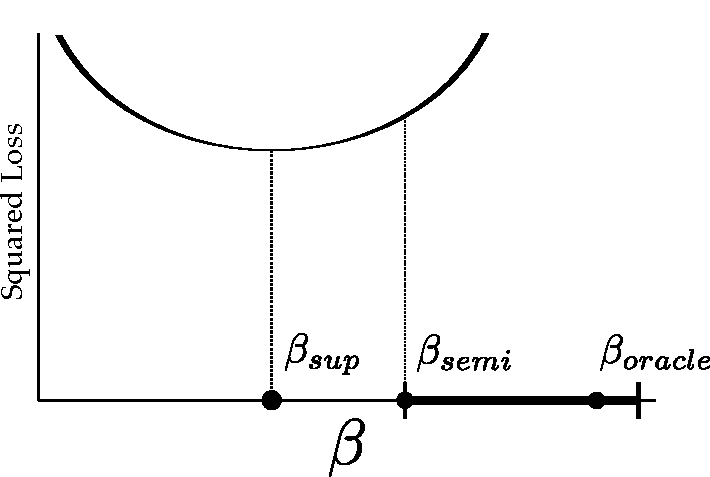
\includegraphics[width=0.8\textwidth]{1Dconstrainedspace.pdf}
  \caption{An example where implicitly constrained optimization improves performance. The supervised solution $\hat{\beta}_{sup}$ which minimizes the supervised loss (shown), is not part of the interval of allowed solutions. The solution that minimizes this supervised loss within the allowed interval is $\hat{\beta}_{semi}$. This solution is closer to the optimal solution ${\beta}^{\ast}$ than the supervised solution $\hat{\beta}_{sup}$.} \label{fig:constrainedproblem}
\end{figure}

Using the set of labeled data, we can construct a supervised solution $\hat{\beta}_{sup}$ that minimizes the loss on the training set of $N_l$ labeled objects, see Figure \ref{fig:constrainedproblem}:

\begin{equation} \label{supervisedsolution}
\hat{\beta}_{sup} = \operatorname*{argmin}_{\beta \in \mathbb{R}} \sum_{i=1}^{N_l} (x_i \beta - y_i)^2
\end{equation}

Now, either this solution falls within the constrained region, $\hat{\beta}_{sup} \in \mathcal{C}_{\boldsymbol{\beta}}$ or not, $\hat{\beta}_{sup} \notin \mathcal{C}_{\boldsymbol{\beta}}$, with different consequences:

\begin{enumerate}
  \item If $\hat{\beta}_{sup} \in \mathcal{C}_{\boldsymbol{\beta}}$ there is a labeling of the unlabeled points that gives us the same value for $\beta$. Therefore, the solution falls within the allowed region and there is no reason to update our estimate. Therefore $\hat{\beta}_{semi}=\hat{\beta}_{sup}$.
  \item Alternatively, if $\hat{\beta}_{sup} \notin  \mathcal{C}_{\boldsymbol{\beta}}$, the solution is outside of the constrained region (as shown in Figure \ref{fig:constrainedproblem}): there is no possible labeling of the unlabeled data that will give the same solution as $\hat{\beta}_{sup}$. We then update the $\beta$ to be the $\beta$ within the constrained region that minimizes the loss on the supervised training set. As can be seen from Figure \ref{fig:constrainedproblem}, this will be a point on the boundary of the interval. Note that $\hat{\beta}_{semi}$ is now closer to $\beta^{*}$ than $\hat{\beta}_{sup}$. Since the true loss function $R^*(\beta)$ is convex  and achieves its minimum in the optimal solution, corresponding to the true labeling, the risk of our semi-supervised solution will always be equal to or lower than the loss of the supervised solution.
\end{enumerate}

Thus, the proposed update either improves the estimate of the parameter $\beta$ or it does not change the supervised estimate. In no case will the semi-supervised solution be worse than the supervised solution, in terms of the expected squared loss. We summarize this result in the following theorem:



The last part of the theorem gives a general condition when, in expectation, our semi-supervised approach will outperform the supervised learner. Because $\hat{\beta}_{semi}$ will never be worse than $\hat{\beta}_{sup}$, to prove this we only need to show that for some observation of a labeled point with positive $f_{X,Y}(x,y)>0$, the estimated $\hat{\beta}_{sup}$ is outside of the interval $\mathcal{C}_{\boldsymbol{\beta}}$, in which case $R^*(\hat{\beta}_{semi}) < R^*(\hat{\beta}_{sup})$. 

If we observe an object labeled $1$ with feature value $x$, the corresponding estimate $\hat{\beta}_{sup}=\tfrac{1}{x}$. Since the improvement in loss will only result if this estimate is not in the constrained region, we need to show that:

\begin{equation} \label{eq:condition}
P(\tfrac{1}{x} \notin \mathcal{C}_{\boldsymbol{\beta}},y=1)>0
\end{equation}

To do this, consider the bounds of the interval $\mathcal{C}_{\boldsymbol{\beta}}$. These most extreme values are obtained whenever all negative values of $x$ are assigned label $0$ while the positive $x$ get labels $1$, or the other way around. From \eqref{eqn:sslsolution} and writing $\mathbb{E}(X^2)=\int_{-\infty}^{\infty} { x^2 f_X(x) \mathrm{d}x}$ we find the interval is given by:  

\begin{equation} \label{eq:condition2}
\mathcal{C}_{\boldsymbol{\beta}}=\left[ \frac{\int_{-\infty}^{0}{x f_X(x) \mathrm{d}x }}{\mathbb{E}(X^2)},\frac{\int_{0}^{\infty}{x f_X(x)  \mathrm{d}x }}{\mathbb{E}(X^2)} \right]
\end{equation}
Combining this with \eqref{eq:condition}, we get the following condition:

\begin{equation} \label{eq:condition3}
P \left( \frac{\mathbb{E}(X^2)}{\int_{-\infty}^{0}{x f_X(x)  \mathrm{d}x }} < x < 0 \vee 0 < x < \frac{\mathbb{E}(X^2)}{\int_{0}^{\infty}{x f_X(x)  \mathrm{d}x }},y=1 \right) > 0
\end{equation}
Since $f_{X,Y}$ is assumed to be continuous, $\mathbb{E}[X^2]>0$ and the lower bound in this equation is always smaller than $0$, while the upper bound is always larger than $0$.  Therefore, \eqref{eq:condition2} holds whenever $f_{X,Y}(0,1)>0$. The assumption of the continuity of $f_{X,Y}$ ensures that  \eqref{eq:condition3} holds.  The property $f_{X,Y}(0,1)>0$ is satisfied by many distributions of the data. The result, therefore, indicates, that in the case of $1$ labeled sample improvement is not only possible, but will occur in many cases. When we have multiple labeled examples, this effect will likely become smaller. This makes sense: the more labeled data we have to estimate the parameter, the smaller the impact of the unlabeled objects will be.

\end{pf}
%The strong result of Theorem 1, that performance \emph{never} gets worse,  holds in the 1D case with unlimited unlabeled data and no intercept in the model. A slightly weaker result, that performance does not degrade \emph{on average} may still hold without these assumptions. The set of classifiers induced by the possible labelings of a large number of unlabeled objects is  likely to contain a better solution than the supervised solution based on limited labeled data alone. By finding the solution within this set that minimizes the loss on the labeled data, we may still, on average, always improve performance.

\section{Empirical Results} 
\label{section:empiricalresults}

The empirical properties of our proposed approach are evaluated in two ways. Firstly, we study the behavior of the error rates of our semi-supervised approach for increasing amounts of unlabeled data. The goal is to study whether the ICLS procedure exhibits the improvement in expectation that motivated this method. Secondly, we compare the classification performance using a cross-validation setup on various datasets to study how the properties of our approach compare to other semi-supervised least squares classification approaches.
% several state-of-the-art semi-supervised methods described in Section \ref{section:relatedwork} on various benchmark datasets.

Since we extended the least squares classifier to the semi-supervised setting, we compare how, for different sizes of the unlabeled sample,  our semi-supervised least squares approach fares against supervised least squares classification (LS) without the constraints. For comparison we included two alternative semi-supervised strategies, namely self-learning applied to the least squares classifier (SLLS) and a procedure were the matrix $\mathbf{X}^T \mathbf{X}$ is replaced by an appropriately scaled matrix $\XeT \Xe$ similar to the estimator in \cite{Shaffer1991}. We will refer to the latter as updated covariance least squares (UCLS) classification. We also included the performance of the least squares classifier if all unlabeled object were to be labeled (LS$_{oracle}$). This serves as the unattainable upper bound on the performance of any semi-supervised learner. 

A description of the datasets used for our experiments is given in Table \ref{table:datasets}. We use datasets from both the UCI repository \cite{Bache2013} and six of the benchmark datasets proposed by \cite{Chapelle2006}. While the benchmark datasets proposed in \cite{Chapelle2006} are useful, in our experience, the results on these datasets are very homogeneous because of the similarity in the dimensionality and their low Bayes errors. The UCI datasets are more diverse both in terms of the number of objects and features as well as the nature of the underlying problems. Taken together, this collection allows us to investigate the properties of our approach for a wide range of problems.

All the code used to run the experiments is available from the first author's website.

\begin{table}[ht] 
\caption{Description of the datasets used in the experiments. Features indicates the dimensionality of the design matrix after categorical features are expanded into dummy variables.}
\begin{center}
\begin{tabular}{rrrr}
  \hline
 Name & \# Objects & \#Features & Source \\ 
  \hline
  Haberman & 306 &   4 & \cite{Bache2013} \\ 
  Ionosphere & 351 &  35 & \cite{Bache2013} \\ 
  Parkinsons & 195 &  23 & \cite{Bache2013} \\ 
  Pima & 768 &   9 & \cite{Bache2013} \\ 
  Sonar & 208 &  61 & \cite{Bache2013} \\ 
  SPECT & 267 &  23 & \cite{Bache2013} \\ 
  SPECTF & 267 &  45 & \cite{Bache2013} \\ 
  Transfusion & 748 &   110 & \cite{Bache2013} \\ 
  WDBC & 569 &  31 & \cite{Bache2013} \\
  Mammography & 961 & 10 & \cite{Bache2013} \\
  Thoraric & 470 & 25 & \cite{Bache2013} \\
  Fertility & 100 & 17 & \cite{Bache2013} \\
  Digit1 & 1500 & 242 & \cite{Chapelle2006} \\ 
  USPS & 1500 & 242 & \cite{Chapelle2006}  \\ 
  COIL2 & 1500 & 242 & \cite{Chapelle2006} \\ 
  BCI & 400 & 118 & \cite{Chapelle2006} \\ 
  g241c & 1500 & 242 & \cite{Chapelle2006} \\ 
  g241n & 1500 & 242 & \cite{Chapelle2006} \\ 
   \hline
\end{tabular}
\end{center}

\label{table:datasets}
\end{table}

\subsection{Comparison of Learning Curves}
We study the behavior of the expected classification error of the ICLS procedure for different sizes for the unlabeled set. As we noted in the introduction, this statistic has two desired properties. First of all it should never be higher than the expected classification error of the supervised solution. Secondly, the expected classification error should not increase as we add more unlabeled data. 

Experiments were conducted as follows. For each dataset, $N_l$ labeled points were randomly chosen, where we make sure it contains at least 1 object from each of the two classes.  With fewer than $m$ samples, the least squares classifier is known to deteriorate in performance as more data is added, a behavior known as peaking \cite{Raudys1998,Opper1996}. Since this is not the topic of this work, we will only consider the situation in which the labeled design matrix is of full rank, which we ensure by setting $N_l=m+5$, the dimensionality and intercept of the dataset plus five observations. For all datasets we ensure a minimum of $N_l=20$ labeled objects.

Next, we create unlabeled subsets of increasing size $N_u=[2,4,8,...,1024]$ by randomly selecting points from the original dataset without replacement. The classifiers are trained using these subsets and the classification performance is evaluated on the remaining objects. Since the test set decreases in size as the number of unlabeled objects increases, the standard error is slightly increases with the number of unlabeled objects.

This procedure of sampling labeled and unlabeled points is repeated $100$ times. We report the mean classification error as well as the standard error of this mean. As can be seen from the tight confidence bands, this offers an accurate estimate of the expected classification error.

% This process of sampling the labeled objects and creating the unlabeled subsets is repeated 100 times and the average classification error and loss on the test set is determined. The latter is done to evaluate whether the approach is effective in increasing generalization performance in terms of the loss used in estimating the classifier. Even though in applications the ultimate goal may typically be classification performance, this allows us to see whether problems occur because of the optimization itself, or because of the link surrogate loss and classification error.

\begin{figure}[ht!] 
  \centering
      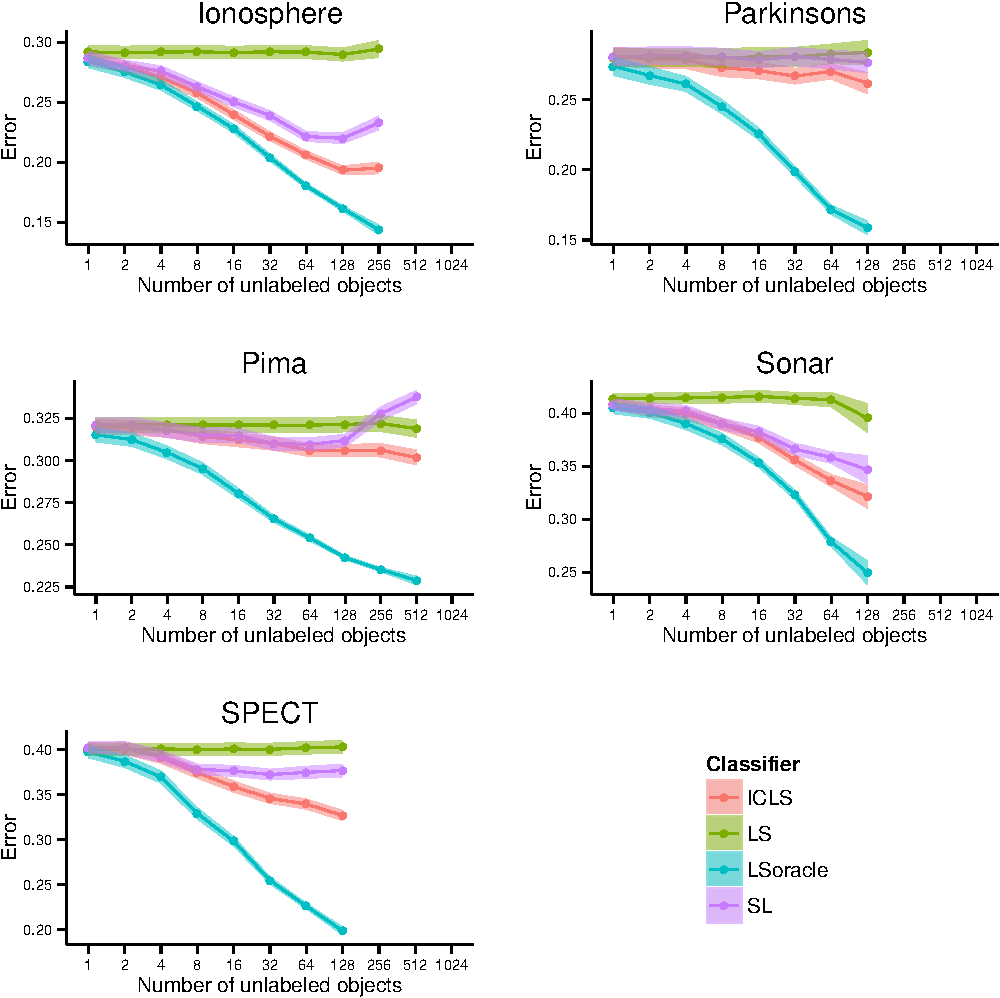
\includegraphics[width=1.0\textwidth]{LearningCurves-1.pdf}
  \caption{Mean classification error for $N_l=\max(m+5,20)$ and $100$ repeats. The error bounds are $+/-$ the standard error of the mean.} \label{fig:learningcurves1}
\end{figure}

\begin{figure}[ht!] 
  \centering
      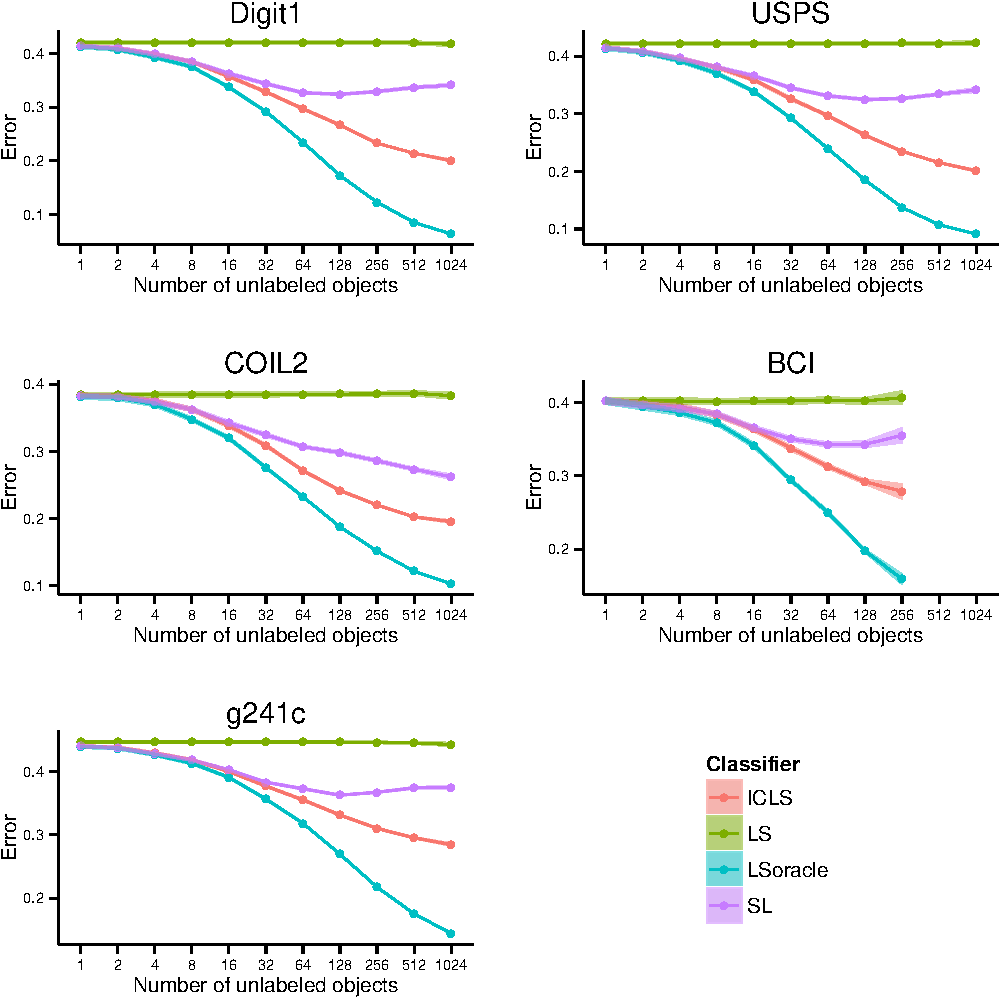
\includegraphics[width=1.0\textwidth]{LearningCurves-2.pdf}
  \caption{Mean classification error for $N_l=\max(m+5,20)$ and $100$ repeats. The error bounds are $+/-$ the standard error of the mean.} \label{fig:learningcurves2}
\end{figure}

The results of these experiments are shown in Figures \ref{fig:learningcurves1} and \ref{fig:learningcurves2}. Note that the error-axis in the figures does not extend to $0$ in order to show the differences between the various methods more clearly.

We find that the ICLS procedure has monotonically decreasing error curves as the number of unlabeled samples increases. Unlike self-learning, there is no deterioration in performance. This is especially apparent, for instance, on the Pima dataset. For the datasets presented in Figure \ref{fig:learningcurves2}, it is interesting to see how the ICLS curves resemble a scaled version of the LS classifier where we assume all data points are labeled. Self-learning does not share this property.

% Also note the difference between the error curves and the loss. It is quite surprising that the loss on the test set decreases in almost every case. Another interesting fact is that the self-learner has similar performance in terms of loss minimization, while its error curves are markedly different.

\subsection{Benchmark performance}
We now consider the cross-validation setting for these datasets. This experiment is set up as follows. For each dataset, the objects are randomly divided into $10$ folds. We iteratively go through the folds using $1$ fold as validation set, and the other $9$ as the training set. From this training set, we then randomly select $N_l=m+5$ labeled objects, as in the previous experiment, and use the rest as unlabeled data. After predicting labels for the validation set for each fold, the classification error is then determined by comparing the predicted labels to the real labels. This is repeated $10$ times, while randomly assigning objects to folds in each iteration.

The cross-validation procedure used here is slightly different from that described in \cite{Chapelle2006}, to make it more closely relate to the cross-validation procedure that is usually employed. More specifically, this procedures ensures the validation sets are independent (non-overlapping), such that, after going over all the folds, each object is in the validation set only once. This is different from the procedure in \cite{Chapelle2006}, were the authors ensure the \emph{labeled} sets or non-overlapping. We have not found a qualitative difference in the error rates, however, when using the procedure proposed in \cite{Chapelle2006}. The advantage of the procedure employed here is that every object gets a single predicted label, allowing for the direct comparison of predictions of different classifiers.

% \begin{table}
\caption{Average 10-fold cross-validation error and standard deviation over 10 repeats. The classifiers that have been compared are supervised Least Squares (LS), Implicitly constrained least squares (ICLS), self-learned least squares (SLLS), updated covariance least squares (UCLS, see text) and for comparison a supervised least squares classifier that has access to all the labels (LSoracle). Indicated in $\mathbf{bold}$ is whether a semi-supervised classifier significantly outperform the supervised LS classifier, as measured using a $t$-test with a $0.05$ significance level. \underline{Underlined} indicates whether a semi-supervised classifier is (significantly) best among the three semi-supervised classifiers considered.} \label{table:cvresults}
\begin{tabular}{l|llllll}
Dataset & LS & ICLS & SLLS & UCLS & LSoracle \\ 
\hline
Haberman & $0.38 \pm 0.03$& $\mathbf{\underline{0.25 \pm 0.00}} $& $0.35 \pm 0.03$& $0.46 \pm 0.09$& $0.35 \pm 0.03$& $0.37 \pm 0.03$\\ 
Ionosphere & $0.21 \pm 0.02$& $\mathbf{\underline{0.14 \pm 0.01}} $& $\mathbf{0.18 \pm 0.02} $& $0.57 \pm 0.02$& $0.20 \pm 0.01$& $\mathbf{0.18 \pm 0.01} $\\ 
Parkinsons & $0.27 \pm 0.02$& $\mathbf{\underline{0.15 \pm 0.00}} $& $\mathbf{0.23 \pm 0.03} $& $0.33 \pm 0.06$& $0.25 \pm 0.02$& $\mathbf{0.24 \pm 0.02} $\\ 
Pima & $0.34 \pm 0.02$& $\mathbf{\underline{0.23 \pm 0.00}} $& $\mathbf{0.31 \pm 0.02} $& $0.37 \pm 0.03$& $0.35 \pm 0.03$& $\mathbf{0.32 \pm 0.01} $\\ 
Sonar & $0.30 \pm 0.03$& $\mathbf{\underline{0.25 \pm 0.01}} $& $0.29 \pm 0.02$& $0.35 \pm 0.03$& $0.30 \pm 0.03$& $0.29 \pm 0.02$\\ 
SPECT & $0.30 \pm 0.03$& $\mathbf{\underline{0.18 \pm 0.01}} $& $\mathbf{0.25 \pm 0.04} $& $0.64 \pm 0.03$& $0.32 \pm 0.03$& $0.29 \pm 0.03$\\ 
SPECTF & $0.33 \pm 0.02$& $\mathbf{\underline{0.24 \pm 0.01}} $& $\mathbf{0.29 \pm 0.02} $& $\mathbf{0.29 \pm 0.04} $& $0.34 \pm 0.02$& $0.34 \pm 0.02$\\ 
Transfusion & $0.35 \pm 0.04$& $\mathbf{\underline{0.23 \pm 0.00}} $& $0.33 \pm 0.04$& $0.53 \pm 0.08$& $0.40 \pm 0.07$& $0.34 \pm 0.04$\\ 
WDBC & $0.11 \pm 0.01$& $\mathbf{\underline{0.04 \pm 0.00}} $& $\mathbf{0.09 \pm 0.01} $& $0.37 \pm 0.04$& $0.09 \pm 0.01$& $\mathbf{0.08 \pm 0.01} $\\ 
\end{tabular}
\end{table}


\begin{table}
\caption{Average 10-fold cross-validation error and standard deviation over 20 repeats. The classifiers that have been compared are supervised Least Squares (LS), Implicitly constrained least squares (ICLS), the extended ICLS presented in section 4.3 (ICLS$_{ext}$), the adapted ICLS procedure from section 4.2 (ICLS$_{adp}$),  self-learned least squares (SLLS), updated covariance least squares (UCLS, see text) and the supervised least squares classifier that has access to all the labels (LS$_{oracle}$). Indicated in $\mathbf{bold}$ is whether a semi-supervised classifier significantly outperform the supervised LS classifier, as measured using a $t$-test with a $0.05$ significance level. \underline{Underlined} indicates whether a semi-supervised classifier is (significantly) best among the three semi-supervised classifiers considered.} \label{table:cvresults}
\begin{tabular}{l|lllllll}
Dataset & LS & ICLS & ICLS$_{ext}$ & ICLS$_{adp}$ & SLLS & UCLS & LS$_{oracle}$ \\ 
\hline
Haberman & $0.36 (0)$& $0.34 (3)$& $0.35 (0)$& $0.35 (8)$& $0.35 (7)$& $0.46 (20)$& $0.26 (0)$\\ 
Ionosphere & $0.28 (0)$& $\mathbf{\underline{0.19 (0)}} $& $\mathbf{0.23 (0)} $& $0.39 (20)$& $\mathbf{0.24 (1)} $& $0.36 (18)$& $0.14 (0)$\\ 
Parkinsons & $0.24 (0)$& $0.24 (9)$& $0.24 (6)$& $0.31 (20)$& $\mathbf{\underline{0.22 (1)}} $& $0.41 (20)$& $0.14 (0)$\\ 
Diabetes & $0.37 (0)$& $\mathbf{\underline{0.33 (0)}} $& $0.36 (1)$& $0.42 (19)$& $0.36 (9)$& $0.42 (19)$& $0.23 (0)$\\ 
Sonar & $0.42 (0)$& $\mathbf{\underline{0.34 (0)}} $& $\mathbf{0.38 (0)} $& $0.42 (11)$& $\mathbf{0.37 (2)} $& $0.44 (15)$& $0.25 (0)$\\ 
SPECT & $0.41 (0)$& $\mathbf{\underline{0.33 (0)}} $& $0.41 (4)$& $0.45 (18)$& $0.40 (7)$& $0.45 (17)$& $0.17 (0)$\\ 
SPECTF & $0.45 (0)$& $\mathbf{\underline{0.35 (0)}} $& $\mathbf{0.42 (2)} $& $0.45 (11)$& $\mathbf{0.40 (1)} $& $0.45 (11)$& $0.23 (0)$\\ 
Transfusion & $0.25 (0)$& $0.25 (14)$& $\underline{0.24 (4)}$& $0.26 (17)$& $0.24 (11)$& $0.34 (20)$& $0.23 (0)$\\ 
WDBC & $0.10 (0)$& $\mathbf{\underline{0.10 (4)}} $& $0.10 (10)$& $0.30 (20)$& $0.10 (10)$& $0.30 (20)$& $0.05 (0)$\\ 
Mammography & $0.31 (0)$& $0.30 (3)$& $0.31 (12)$& $0.37 (20)$& $0.32 (13)$& $0.41 (20)$& $0.20 (0)$\\ 
Thoraric & $0.27 (0)$& $0.26 (5)$& $0.26 (2)$& $0.35 (20)$& $\mathbf{\underline{0.24 (1)}} $& $0.35 (20)$& $0.17 (0)$\\ 
Fertility & $0.28 (0)$& $\mathbf{\underline{0.24 (4)}} $& $0.27 (3)$& $0.31 (16)$& $\mathbf{0.25 (3)} $& $0.37 (18)$& $0.13 (0)$\\ 
Digit1 & $0.42 (0)$& $\mathbf{\underline{0.20 (0)}} $& $\mathbf{0.38 (0)} $& $0.44 (15)$& $\mathbf{0.35 (0)} $& $\mathbf{0.40 (6)} $& $0.06 (0)$\\ 
USPS & $0.42 (0)$& $\mathbf{\underline{0.20 (0)}} $& $\mathbf{0.38 (0)} $& $0.44 (19)$& $\mathbf{0.34 (0)} $& $\mathbf{0.39 (2)} $& $0.09 (0)$\\ 
COIL2 & $0.38 (0)$& $\mathbf{\underline{0.20 (0)}} $& $\mathbf{0.35 (0)} $& $0.44 (20)$& $\mathbf{0.27 (0)} $& $0.40 (17)$& $0.10 (0)$\\ 
BCI & $0.41 (0)$& $\mathbf{\underline{0.27 (0)}} $& $\mathbf{0.36 (0)} $& $0.40 (9)$& $\mathbf{0.35 (0)} $& $0.42 (12)$& $0.16 (0)$\\ 
g241c & $0.44 (0)$& $\mathbf{\underline{0.28 (0)}} $& $\mathbf{0.41 (0)} $& $0.43 (5)$& $\mathbf{0.39 (0)} $& $\mathbf{0.43 (5)} $& $0.14 (0)$\\ 
g241n & $0.45 (0)$& $\mathbf{\underline{0.28 (0)}} $& $\mathbf{0.41 (0)} $& $\mathbf{0.44 (2)} $& $\mathbf{0.39 (0)} $& $\mathbf{0.42 (1)} $& $0.13 (0)$\\ 
\end{tabular}
\end{table}

The results shown in Table \ref{table:cvresults} tell a similar story to those in the previous section. Most importantly for the purposes of this paper, ICLS, in general, offers solutions that give at least no higher expected classification error than the supervised procedure. On these datasets, the self-learning approach seems to share this property. However, if we look at for how many of the cross-validation repeats the ICLS and self-learning give lower error than the supervised solution, there is a clear difference. The self-learning solution gives a higher error on more of the repeats than ICLS, for most of the datasets. The results also show that unlabeled information can be of use. Particularly on the last six datasets, ICLS offers large improvement in classification accuracy over the supervised solution. The differences in performance between ICLS and self-learning can also be quite substantial, where ICLS outperforms self-learning on most of the datasets.

UCLS often shows major deterioration in performance. It does show some minor improvements on some of the SSL benchmark datasets, in particular USPS, g241c and g241n. In the latter cases, improvements are small. It is unclear whether these effects are real, given the small deterioration in performance on related datasets.

% Similar to \cite{Chapelle2006}, we choose to compare our linear method to state-of-the-art linear semi-supervised classifiers. In this case, this means logistic regression and entropy regularization proposed by \cite{Grandvalet2005}, the linear support vector machine and its Transductive SVM as implemented by \cite{Sindhwani2006}, and self-learning applied to these two supervised classifiers.

% To evaluate the performance of the different methods, the datasets were divided in $\tfrac{n}{(m+2)}$ folds, following the same argument as in the first experiment. Sequentially, each fold was used for training, while the rest of the data were used as both unlabeled data and as the test set. This is therefore a transductive learning setting. The setup is similar to \cite{Chapelle2006}, but with more folds used. The averaged classification errors over all folds can be found in Table \ref{table:cvtable}.

% latex table generated in R 2.15.2 by xtable 1.7-0 package
% Mon Apr 22 21:43:10 2013
% \begin{table}[ht] \label{table:results}
% \caption{The results comparing the proposed technique to alternatives on several benchmark datasets. Least Squares Classifier (LS), Implicitly Constrained Least Squares Classifier (ICLS), Self Learning Least Squares Classifier (SLLS),  Logistic Regression(LR), Entropy Regularized Logistic Regression (ERLR), Self Learning Logistic Regression (SLLR), Linear Support Vector Machine (SVM), Transductive Support Vector Machine (TVM), Self Learning Support Vector Machine (SLSVM). Bold results indicate the lowest error on a dataset for compared to other versions of the same classifier (LS, LR or SVM). Note ICLS is always best among the LS classifiers, while this does not hold for the semi-supervised versions of the LR or SVM.}


% \begin{center}
% \begin{tabular}{l|lll|lll|lll}
%   \hline
%  & LS & ICLS & SLLS & LR & ERLR & SLLR & SVM & TSVM & SLSVM \\ 
%   \hline
% Haberman & 0.37 & \textbf{0.35} & \textbf{0.35} & \textbf{0.28} & 0.35 & \textbf{0.28} & 0.35 & 0.39 & \textbf{0.34} \\ 
%   Ionosphere & 0.34 & \textbf{0.20} & 0.28 & 0.29 & \textbf{0.26} & 0.33 & \textbf{0.21} & 0.26 & \textbf{0.21} \\ 
%   Parkinsons & 0.28 & \textbf{0.27} & 0.30 & \textbf{0.25} & 0.30 & \textbf{0.25} & \textbf{0.22} & 0.23 & \textbf{0.22} \\ 
%   Pima & 0.41 & \textbf{0.34} & 0.41 & 0.42 & \textbf{0.41} & 0.43 & \textbf{0.34} & 0.45 & \textbf{0.34} \\ 
%   Sonar & 0.41 & \textbf{0.33} & 0.39 & 0.50 & \textbf{0.31} & 0.50 & \textbf{0.27} & 0.42 & \textbf{0.27} \\ 
%   SPECT & 0.46 & \textbf{0.34} & 0.44 & \textbf{0.21} & 0.25 & \textbf{0.21} & 0.28 & \textbf{0.23} & 0.28 \\ 
%   SPECTF & 0.45 & \textbf{0.39} & 0.42 & \textbf{0.21} & 0.79 & \textbf{0.21} & \textbf{0.25} & 0.42 & \textbf{0.25} \\ 
%   Transfusion & 0.36 & \textbf{0.32} & 0.36 & \textbf{0.26} & 0.34 & \textbf{0.26} & 0.32 & 0.37 & \textbf{0.31} \\ 
%   WDBC & 0.38 & \textbf{0.37} & \textbf{0.37} & 0.48 & \textbf{0.44} & 0.48 & \textbf{0.08} & 0.15 & \textbf{0.08} \\ 
%   Digit1 & 0.39 & \textbf{0.20} & 0.34 & 0.50 & \textbf{0.07} & 0.50 & 0.08 & \textbf{0.08} & \textbf{0.08} \\ 
%   USPS & 0.38 & \textbf{0.20} & 0.33 & 0.20 & \textbf{0.11} & 0.20 & \textbf{0.12} & 0.23 & \textbf{0.12} \\ 
%   COIL2 & 0.36 & \textbf{0.21} & 0.27 & \textbf{0.47} & 0.49 & 0.50 & 0.17 & \textbf{0.15} & 0.17 \\ 
%   BCI & 0.47 & \textbf{0.32} & 0.47 & 0.41 & \textbf{0.33} & 0.40 & \textbf{0.30} & 0.35 & \textbf{0.30} \\ 
%   g241c & 0.45 & \textbf{0.29} & 0.40 & 0.17 & \textbf{0.16} & 0.43 & 0.23 & \textbf{0.17} & 0.23 \\ 
%   g241n & 0.47 & \textbf{0.28} & 0.42 & 0.22 & \textbf{0.17} & 0.50 & 0.23 & \textbf{0.18} & 0.23 \\ 
%    \hline
% \end{tabular}

% \end{center}
% \end{table}



% Note that the \emph{supervised} linear support vector machine outperforms most other methods on many of the datasets. The semi-supervised SVM, however, is much less stable and on some datasets, has worse performance. This is not the case for our approach, which is always the preferred approach among the least squares classifiers.

\section{Discussion}
The theoretical result in Section 4 shows that projecting onto the constrained subset $\Cb$ leads to improvement in terms of squared loss (Theorem 1 and 3) and in terms of Euclidean distance of the parameter estimate (Theorem 2). These results are encouraging in the light of negative theoretical performance results in the semi-supervised literature \cite{Cozman2006}. The empirical results in the previous section indicate that in terms of the expected classification error, ICLS never significantly deteriorates with increasing amounts of unlabeled data on this collection of datasets. These empirical observations are all the more interesting considering that the loss evaluated in Section 5 is misclassification error and not the squared loss that was considered in Theorem 1 and 3 or the Euclidean parameter distance of Theorem 2. Furthermore the experiments were carried out on limited unlabeled data, not the unlimited setting considered in the theorems. This indicates that projecting onto the subset $\Cb$, leads to a semi-supervised learner with desirable behavior, both theoretically in terms of various measures of risk and empirically in terms of classification error.

It has been argued that, for discriminative classifiers, semi-supervised learning is impossible without additional assumptions about the link between labeled and unlabeled objects \cite{Seeger2001,Singh2008}. ICLS, however, is both a discriminative classifier and no explicit additional assumptions about this link are made. Any assumptions that are present follow, implicitly, from the choice of squared loss as the loss function and from the hypothesis space. One could argue that constraining the solutions to $\Cb$ is an assumption as well. While this is true, it corresponds to a very weak assumption about the supervised classifier: that it will improve when we add additional labeled data. This lack of additional assumptions has another advantage: no additional parameters need to be correctly set for the results in Sections 4 and 5. There is, for instance, no weight to be chosen for the importance of the unlabeled data. Therefore, implicitly constrained semi-supervised learning is a very different approach to semi-supervised learning than the methods discussed in Section 2.

The quadratic programming formulation of ICLS presented in Section 3 allows one to use the standard and constantly improving tools from convex optimization to find the ICLS estimate. Unfortunately one has to go from a convex problem with $m$ variables in the supervised case to a constrained convex problem with $N_u$ variables for ICLS. For very large $N_u$, this may not currently be computationally feasible. Improvements in quadratic programming solvers may help alleviate this problem. Additionally, instead of finding the exact optimal labeling $\mathbf{y}_u$, as was employed in our experiments, approximations to these optima may take less time to compute without having a large effect on the final estimate of $\boldsymbol{\hat{\beta}}_{semi}$.

Compared to ICLS, self-learning is much more favorable in terms of computational cost. Self-learning usually converges in a few iterations, where each iteration has the cost of one supervised least squares estimation. As we noted in Section 5 the self-learning approach can increase performance, but large amounts of unlabeled data can also have a detrimental effect. Also, the performance of ICLS is significantly better on many of the datasets considered in our experiments. Hence the price one pays for the low computational cost is in terms of classification error. Note that the solution provided by self-learning is, by construction, also in the constrained subset $\Cb$. The difference with ICLS is that in ICLS the choice of estimate from $\Cb$ is based on information of the labeled objects only, while SLLS also uses the imputed labels on the unlabeled objects. This may lead to self-deception: if the imputed labels are wrong, a good fit for these wrongly imputed labels does not necessarily lead to a good estimate of $\boldsymbol{\beta}$.

The plug-in version of the LS, UCLS, while fast and intuitive, does not perform well. We found that it only offers some improvement on datasets with low Bayes error. This does not correspond to the observations of \cite{Shaffer1991} that the covariance update only decreases the parameter value in high noise settings. While we do not currently fully understand this behavior, it may be related to the finite sample estimate of $\mathbb{E}[\mathbf{X}'\mathbf{X}]$ that we consider or the differences in modeling assumptions when going from the regression setting considered in \cite{Shaffer1991} to the classification setting considered here.

The alternative distance measures used for the projection onto $\Cb$ and introduced in section 4 did not give rise to the same increase in performance in terms of classification error as the original ICLS procedure. This was to be expected for the Euclidean distance measure, since the corresponding objective that is minimized is potentially far removed from the goal of classification. It is interesting, however, that the distance measure used in ICLS$_{extended}$, which does offer the strong theoretical guarantees in terms of the loss function, gives rise to behaviour that is perhaps too conservative. In terms of robustness, this classifier corresponds most directly to our goal of constructing a semi-supervised version that is never worse than the supervised alternative. In terms of performance in practice, however, less conservative projections, such as the original ICLS may strike a better balance between robustness and improvement in performance.

In Figure 1, we illustrate that projecting onto the subset $\Cb$ causes improvement as long as a better solution $\hat{\beta}_{oracle}$ than the supervised solution is within $\Cb$. A smaller $\Cb$ will give a larger improvement, since the projection is going to be closer to $\hat{\beta}_{oracle}$. In the extreme case where only $\hat{\beta}_{oracle}$ forms the subset, this clearly gives a great improvement over supervised learning. It therefore makes sense to think about reducing the size of $\Cb$. In the approach presented in this work, however, to ensure a better solution $\hat{\beta}_{oracle}$ than the supervised solution is always within the constrained set with probability $P(\hat{\beta}_{oracle} \in \Cb)=1$, our choice of $\Cb$ is conservatively large. It contains elements corresponding to all labelings of the unlabeled points,  even extremely unlikely ones. By excluding unlikely labelings from the subset, the size of $\Cb$ may shrink, while the probability that it includes $\hat{\beta}_{oracle}$ remains high. For instance, one might exclude labelings with class priors that are very unlikely to occur, given the class priors that are observed in the labeled data, a strategy which is also employed in Transductive SVMs where it is necessary to converge to meaningful local optima. Changes to $\Cb$ may, therefore, allow for larger improvements in terms of the risk or classification error, while introducing a small chance of deterioration in performance.

While the results presented in this work are promising for squared loss, a worthwhile extension would be to other loss functions. In this work, we were able to derive a quadratic programming formulation for ICLS because there is a closed-form solution of the supervised least squares problem. For many loss functions, closed-form solutions do not exist, which prohibits a straightforward formulation of their implicitly constrained semi-supervised counterparts. In particular, in the derivation of ICLS, we made use of the closed-form solution given an imputed labeling to derive a quadratic programming problem in terms of the labels. Without such a solution, one of the main difficulties is that, even if the loss considered is differentiable, one cannot straightaway apply techniques like gradient descent to the parameters as this typically leads to solutions that are outside of the set $\Cb$. 

Besides these issues, there is the other open question of what loss functions could benefit from constraining the solution to a subset like $\Cb$ in the first place. For logistic loss, for instance, the use of the logistic function ensures that posteriors are always between $[0,1]$. In that case it seems that the current definition of $\Cb$ does not constrain the solutions at all. Treating negative log likelihood as a loss function, on the other hand, does lead to interesting semi-supervised classifiers, for instance in linear discriminant analysis \cite{Krijthe2014}. Even when $\Cb$ does not constrain the solution, we could still be able to construct other constrained sets with interesting performance guarantees. For instance, many semi-supervised classifiers make the additional assumption that the mean posterior labeling of the unlabeled objects is similar to the observed label prior in the labeled objects \cite{Joachims1999,Collobert2006} or is assumed to be known \cite{Mann2010}. Rather than ensuring non degradation for every transductive set, such as the result in Theorem 3, such additions to the definition of $\Cb$ could lead to improvement over the supervised solution with high probability.

Finally, a rather interesting application of the idea presented here is to semi-supervised regression. \cite{Culp2008} argues that in least squares regression, unlabeled data may not help. But assuming bounded outputs, which may be justified in certain settings, our approach can again provide improvement guarantees.

% While the results presented in this work promising for squared loss, in its current form, it can be shown that the approach does not work for some other losses.  For instance, for monotonically decreasing loss function, such as the hinge or logistic loss used, respectively, in support vector classification and logistic regression, the approach does not seem to offer any improvement. For these types of losses, we can always find a labeling such that the loss is minimized at the supervised solution. In other words, the supervised solution is always within $\Cb$. For these types of classifiers, we need to additionally shrink the constrained space to allow for improvements. Fortunately, a lot of interesting classifiers still allow for the implicitly constrained semi-supervised learning approach to be applied. For instance, many classifiers based on a maximum likelihood formulation. In this way, the procedure offers an interesting alternative to Expectation Maximization based approaches like self-learning, given its convex loss function and robustness to misspecification.

% In many cases the improvements were substantial. It is possible that alternative semi-supervised techniques may perform even better on some of these datasets. As we noted in Section 2, however, these are not based on least squares loss and hence are not a semi-supervised version of least squares classification. Moreover, they do not offer the same improvement in expectation that we have attempted to ensure here. Regardless of the size of the improvement, perhaps the most surprising conclusion is that this novel type of semi-supervised method works at all. This is surprising, first of all because we 

% Alternatively, one could argue it is unsurprising ICLS works, since the model does not fit the data and we do not use any form of regularization on the parameter values. Most models used in practice do not directly minimize the ultimate goal of minimizing misclassification. For computational reasons, often convex surrogate losses, such as the one employed here are minimized. We have chosen to restrict ourselves to a particular convex loss and attempted whether we could ensure improvement in terms of this chosen loss function. As for regularization, the proposed method can easily be extended to include a regularization term. This would, however, introduce an additional parameter to be set by the user. On of the advantages of ICLS is that it is a type of data dependent regularization, and no additional parameter value needs to be selected. In our experience, ICLS combined with regularization still outperforms regularized supervised learning, although the differences become smaller.

% There are several simple ways in which the speed of ICLS could be improved. Firstly, whereas we initialize the gradient descent by soft labeling all objects as $0.5$, better initializations are likely possible. For instance, we may use the self-learning solution or a labeling given by the supervised solution. Secondly, it may not be necessary to solve the minimization exactly. While this gives precise values for the imputed labels, early termination of the gradient descent may not have much effect on the estimation of $\mathbf{\beta}$.

% Another interesting observation is the occurrence of the peaking phenomenon \cite{Raudys1998,Opper1996} in this semi-supervised setting, see for example, the learning curves on the COIL2 and BCI datasets. While this has been observed for learning curves of the number of labeled samples, here we find it also occurs when we change the number of unlabeled samples. It also seems that for some datasets ICLS is more sensitive to this problem than self-learning. As yet, we do not have any explanation for this behavior.  Further improvements to the current approach may start by trying to understand this occurrence of peaking.

These results are all the more interesting once we compare the total squared loss on the test set. Here, ICLS and self-learning seem to offer similar performance. This is quite unexpected and unlike the results in, for instance \cite{Loog2010,Loog2012a}, where the self-learner  often performed much worse in terms of the loss than an approach based on constraining the solution. The difference may be explained by the fact that the discriminative classifier used here is less susceptible to this problem than the generative approaches in \cite{Loog2010,Loog2012a}.

%The robustness of the method comes from the fact that we do not accept solutions that do not work on the labeled data. The goal of semi-supervised learning is to improve supervised techniques using the additional information inherent in the additional unlabeled objects. Previous approaches have done this by changing the loss function that is being optimized by introducing an extra term corresponding to assumptions about the unlabeled data. The loss function then becomes a mixture between the supervised objective and an unsupervised objective. If the goal is supervised learning, we propose that the loss function should remain the supervised loss function. The unlabeled objects are used to introduce constraints on the possible solutions to this loss function, but does not change its shape.  

%In those cases, our approach is clearly helpful. In our experience, the performance increase of unlabeled data is reduced as we set the regularization parameter. In the small sample case, we may not be able to accurately set this parameter, so the unlabeled data may still be preferable.

%Extension to other methods. The challenge here is to solve the resulting optimization problem.  Given the desirable properties of our approach, an interesting extension would be an implicitly constrained variant of the support vector machine, or logistic regression. Because of the closed work solution of the supervised linear least squares model \eqref{}, in our formulation we could plug in this solution in the semi-supervised problem. In general, this is not possible. Another issue is whether there are any implicit constraints that can be leveraged by the unlabeled objects. For instance, when we allow fractional labelings for the unlabeled data in logistic regression, we can always find a labeling that corresponds to the supervised solution. Things chance if we do not allow for fractional labelings.

\section{Conclusion}
This contribution introduced a new semi-supervised approach to least squares classification. By implicitly considering all possible labelings of the unlabeled objects and choosing the one that best matches the labeled observations, we derived a robust classifier through a simple quadratic programming formulation. For this procedure, in the univariate setting with a linear model without intercept, we can prove it never degrades performance in terms of squared loss (Theorem 1). Experimental results indicate that in expectation this robustness also holds in terms of classification error on real datasets. Hence, semi-supervised learning for least squares classification without additional assumptions can lead to improvements over supervised least squares classification both in theory and in practice.

\section*{Acknowledgements}
Part of this work was funded by project P24 of the Dutch public-private research community COMMIT.

% The Appendices part is started with the command \appendix;
% appendix sections are then done as normal sections
% \appendix

% \section{}
% \label{}

% Bibliographic references with the natbib package:
% Parenthetical: \citep{Bai92} produces (Bailyn 1992).
% Textual: \citet{Bai95} produces Bailyn et al. (1995).
% An affix and part of a reference:
%   \citep[e.g.][Ch. 2]{Bar76}
%   produces (e.g. Barnes et al. 1976, Ch. 2).
\bibliography{clean}
\bibliographystyle{plainnat}
% 
% \begin{thebibliography}{}
% 
% % \bibitem[Names(Year)]{label} or \bibitem[Names(Year)Long names]{label}.
% % (\harvarditem{Name}{Year}{label} is also supported.)
% % Text of bibliographic item
% 
% \bibitem[]{}
% 
% \end{thebibliography}

\end{document}

